\usepackage{tikz}
\usetikzlibrary{shapes,positioning}
    
    \tikzset{
        nodelabel/.style = {draw=none, rectangle, font=\small},
        edgeleft/.style = {draw=mustard, line width=1pt},
        edgeright/.style = {draw=lightpurple, line width=1pt},
        edgelabelleft/.style = {midway, above right=1.5pt, color=mustard},
        edgelabelright/.style = {midway, above left=1.5pt, color=lightpurple}
    }
    \definecolor{mustard}{HTML}{f08c00}
    \definecolor{lightpurple}{HTML}{9c36b5}
    \begin{figure}[H]
        \centering
        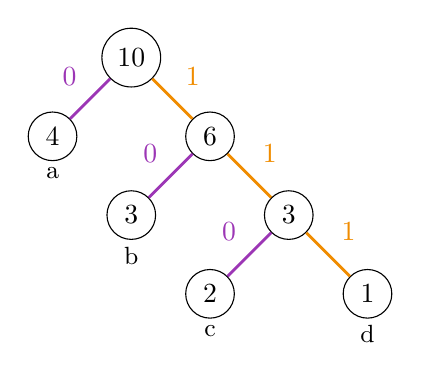
\begin{tikzpicture}
            \node[circle, draw] (A) at (1, 4) {10};
            \node[circle, draw] (B) at (0, 3) {4};
            \node[circle, draw] (C) at (2, 3) {6};
            \node[circle, draw] (D) at (1, 2) {3};
            \node[circle, draw] (E) at (3, 2) {3};
            \node[circle, draw] (F) at (2, 1) {2};
            \node[circle, draw] (G) at (4, 1) {1};

            \draw[edgeright] (A) -- (B) node[edgelabelright] {0};
            \draw[edgeleft] (A) -- (C) node[edgelabelleft] {1};
            \draw[edgeright] (C) -- (D) node[edgelabelright] {0};
            \draw[edgeleft] (C) -- (E) node[edgelabelleft] {1};
            \draw[edgeright] (E) -- (F) node[edgelabelright] {0};
            \draw[edgeleft] (E) -- (G) node[edgelabelleft] {1};
            
            \node[nodelabel, below=-1pt of G] {d};
            \node[nodelabel, below=-1pt of F] {c};
            \node[nodelabel, below=-1pt of D] {b};
            \node[nodelabel, below=-1pt of B] {a};
        \end{tikzpicture}
        \label{fig:huffman_graph}
        \caption{Árbol de Huffman para la cadena $S=\text{abcdabcaba}$}
    \end{figure}